\documentclass[a4paper]{article}
\title{Praktikrapport - Universal Robots}
\author
{
    Johannes Ehlers Nyholm Thomsen\\ 
    \texttt{joha321j@edu.ucl.dk}
}

% Danish symbols.
\usepackage[utf8]{inputenc}
\usepackage[danish]{babel}
\usepackage[T1]{fontenc}

% Links and clickable ToC
\usepackage{hyperref}

% Images
\usepackage{graphicx}

\begin{document}

\maketitle

\newpage

\tableofcontents

\newpage

\section{Indledning}

\newpage
\section{Forventninger}
Som led i datamatikeruddannelsen var jeg i et praktikforløb hos Bankdata.
I det praktikforløb blev jeg en del af et udviklingsteam,
hvor jeg hjalp dem med deres projekter.

Inden praktikforløbet hos Universal Robots(UR) startede, havde jeg en forventing om,
at det ville forløbe på samme måde.
Jeg så frem til at arbejde i et område,
der ikke var lige så konservativt som finansverdenen.
Jeg havde specifikt gået efter et firma,
der arbejdede i en anden sektor end Bankdata for at få et bredere syn på,
hvad jeg ville kunne arbejde med, når jeg var færdiguddannet.

\subsection{Læringsmål}
Jeg har haft opstillet nogle mål for, 
hvad jeg gerne ville have ud af mit praktikforløb hos UR.
Målene har hjulpet mig med at klargøre over for mig selv,
hvad jeg har af forventninger til mig selv under praktikforløbet.

I store træk gik læringsmålene ud på, 
at jeg gerne ville blive bedre til at være en del af et professionelt
udviklingsteam.

\subsubsection*{Personlige Læringsmål}
\label{personligelaeringsmaal}
\begin{itemize}
    \item Få mere erfaring i at indgå fagligt og professionelt i en 
    softwareudviklingsvirksomhed
    \item Forbedre mine evner i at deltage i et professionelt selvstyrende 
    udviklingsteam
    \item Få erfaring med brug af \href{https://en.wikipedia.org/wiki/OKR}{OKRs}
     til at opsætte og organisere mit teams mål for vores produkt.
\end{itemize}

\subsubsection*{Tekniske Læringsmål}
Mine tekniske læringsmål er opstillet på baggrund af en liste af teknologier
som teamet, jeg ville blive en del af, brugte.

\begin{itemize}
    \item Forbedre mine evner som full stack udvikler i .NET teknologi stacken
    \begin{itemize}
        \item Rest API udvikling med ASP.NET Core
        \item Single page application(SPA) udvilking med Blazor
        \item Brug af Entity Framework som Object Relational Mapper(ORM)
    \end{itemize}
    \item Forbedre mine evner inden for OpenAPI dokumentation ved brug af
    Swagger
    \item Få erfaring og kompetencer inden for brug af Elasticsearch
    \item Få erfaring inden for brug af MongoDB
\end{itemize}

Som alle ved overlever en god plan ikke længere end første møde med fjenden,
og jeg har derfor ikke opnået alle de læringsmål, som jeg har beskrevet her.
Se afsnit \ref{praktikforloeb} for en forklaring på hvorfor.
Dog har jeg lært en helt masse andet, 
som jeg vil komme ind på i afsnit \ref{udbytte}.

\newpage
\section{Praktikforløbet}
\label{praktikforloeb}
I dette afsnit vil jeg beskrive selve praktikforløbet.
Først vil jeg beskrive, hvordan den daglige organisering var.
Dernæst vil jeg beskrive de teknologier vi brugte og komme med eksempler på arbejdsopgaver.

\subsection{Eget produktteam}
\label{produktteam}
På første dag i praktikken blev jeg indformeret om,
at jeg ikke ville blive en del af myUR - Fleet.
myUR - Fleet er det produktteam, som jeg fik at vide under praktikinterviewet,
at jeg ville blive en udvikler hos.

I stedet fik Kasper, Mike og jeg at vide,
at vi 3 ville lave vores eget produktteam.
Dernæst fik vi en problemstilling, som vi skulle løse.

\subsubsection{Problemstilling}
Universal Robots er inden for det sidste år skiftet struktur til at være 
produkt-orienterede i stedet for projektorienterede.
I den forbindelse har de forsøgt at give deres teams mere selvstyre ved at 
adoptere OKRs.

Kort fortalt går OKRs ud på, 
at den øverste ledelse sætter overordnede mål for virksomheden.
Ud fra de mål sætter afdelingerne mål for,
hvordan de kan hjælpe ledelsen med at opnå deres mål.
Til sidst sætter produktteamene mål for, 
hvordan de kan hjælpe deres afdeling med at opnå afdelingens mål.
På denne måde har produktteamet selv ansvar for,
hvordan de giver værdi til virksomheden.

En del af OKRs er key results. 
Key results er målbare resultater, der skal bruges til at se,
om produktteamet er på vej mod deres mål.

Problemet var, at der var ingen god måde at visualisere 
fremskridtene for produtkteamene.
Derfor var det svært for teamene og se, hvordan det går med at opnå deres mål.

\subsubsection{Løsning}
I samarbejde med vores mentor, Julian, blev vi enige om, at vi skulle lave en 
løsning, der kunne tage i mod data og visualisere det i form af 
grafer, tabeller og lign.

\subsection{Organisering}
\label{organisering}
Julian og hans kollega Dennis ville være vores produkt owners,
mens vores chef Mark ville være vores stakeholder.
Ellers var Kasper, Mike og jeg fuldstændigt selvstyrende.

\subsubsection{Internt i teamet}
Vi fik et confluence rum, som vi har brugt til at dele forskellige filer, 
domæne modeller og wireframes blandt andet.

\begin{figure}[ht!]
    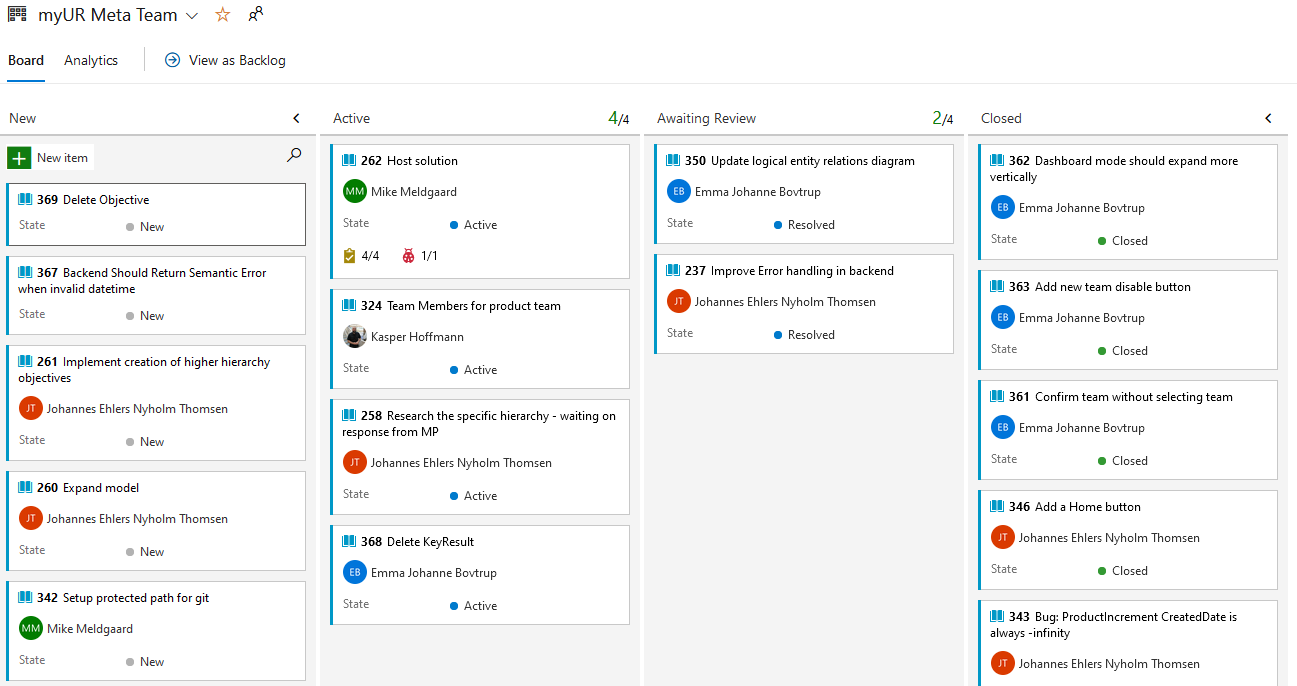
\includegraphics[width=\linewidth]{kanbanboard.png}
    \centering
    \label{kanban}
    \caption{Eksempel på vores kanban board}
\end{figure}

Til den daglige styring og organisering af vores arbejde
har vi brugt en Azure DevOps portal.
Vi brugte et Azure Board som et kanban-board
til at organisere det daglige arbejde, se figur \ref{kanban}.

Vi holdte daglige stand up møder.
Og hver anden uge holdte vi et retrospektiv for at sikre,
at vi blev ved med at blive bedre til at arbejde sammen.

Vi opstillede også kodestandarder, som vi lagde på confluence.
På den måde ville alle i teamet have adgang til dem,
og vi kunne også nemt løbende opdatere dem.
En del af vores standarder var,
at alt kode skal reviewes af et andet teammedlem.
For at sikre det opstillede vi regler,
så der ikke kunne pushes direkte til vores main branch.

\subsubsection{Resten af UR}
Jeg skal indrømme, at da jeg først hørte,
at vi ville blive vores eget selvstændige hold,
var jeg bange for,
at vi ville blive parkeret i et hjørne og glemt indtil de 3 måneder var gået.
Heldigvis gjorde Mark, Julian og Dennis det hurtigt klart for mig,
at jeg tog fejl.

Julian og Dennis deltog i vores daglige stand ups.
Der var de begge rigtigt gode til at komme med deres syn på løsninger til blokerende opgaver.

Julian arrangerede også, at vi holdte en demo hver anden uge.
Under demoen kom de med feedback og idéer til forbedringer for vores produkt.
Mark deltog også i demoerne.

Vores afdeling af UR holdte også et all-hands møde en gang i kvartalet,
hvor hvert team præsenterede, hvad de arbejdede med.
Det skulle vi også,
og til mødet var der stor interesse for vores produkt.

\subsection{Full Stack udvilking}
Da vi var et selvstændigt udvilkingsteam betød det også,
at vi havde ansvaret for alt udvikling af vores produkt
lige fra frontend til database.

\subsubsection{Teknologi Valg}
\label{teknologi_valg}
Det første vi skulle gøre var at blive enige om,
hvilke teknologier vi ville bruge.
Til dette var Julian og Dennis en stor hjælp som sparingspartnere.
Det var nemmere at tage valgne,
når de kunne fortælle,
hvad der blev brugt i virksomheden.
Det handlede om at vælge det rigtige værktøj til opgaven,
men når vi stod med 2 lige gode værktøjer,
var det oplagt at bruge det samme værktøj som vores kollegaer.

\paragraph{Database}
Som database havde vi først tænkt på at bruge en MongoDB dokument database.
Det blev dog tydeligt for os, da vi satte os mere end i vores problemdomæne,
at vores data havde for mange relationer til, at det ville blive en success.

Derfor valgte vi at bruge en SQL database.
Tidligt i udvilkingsforløbet brugte vi blot en SQLite database.
Vi var dog nød til at gå væk fra en SQLite database,
da dens integration med Grafana ikke er særligt god.

I stedet valgte vi at bruge en PostgreSQL database.
Julian og Dennisses team var igang med at migrere fra en MongoDB til en PostgreSQL.
Derfor valgte vi at bruge det i stedet for et af alternativerne,
så det var nemt at udveksle erfaringer med dem.

\paragraph{Backend}
Det var oplagt at bruge .NET til vores backend,
da det blev brugt i resten af URs webløsninger.
Derfor ville vi have rig mulighed for at få hjælp
og udveksle erfaringer med de andre teams.

Som ekstra bonus var det et sprog, 
vi alle tre havde rig erfaring med at bruge grundet vores uddannelse.

\paragraph{Frontend}
Til frontenden valgte vi at bruge Blazor.
Vi valgte det,
da vi alle tre tidligere på uddannelsen havde arbejdet med Razor Pages,
og derfor havde vi erfaring med at bruge C\# til at skrive frontend.

Vi følte heller ikke, at det ville give et bedre produkt for UR,
hvis vi gav os igang med at lære at bruge Angular, React eller Vue.js.

\paragraph{Tye}
For at gøre det nemmere for os at udvikle en distribueret applikation
valgte vi at bruge et værktøj, der hedder
\href{https://github.com/dotnet/tye}{Tye}.
Tye gjorde det meget nemmere for os at udvikle,
da det selv kunne køre vores applikationer op med én kommando.
Alt hvad var nødvendigt var,
at vi havde lavet en yaml fil,
hvor vi fortalte Tye,
hvilke applikationer skulle køres op.
Et udsnit af vores yaml fil kan ses på figur \ref{tye}.

\begin{figure}[ht!]
    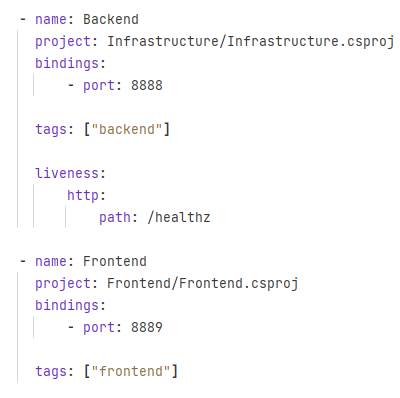
\includegraphics[scale=0.7]{tye.png}
    \centering
    \label{tye}
    \caption{Uddrag af vores tye.yml fil}
\end{figure}

Tye understøttede også hotreloading både af vores frontend og backend,
da begge var .NET applikationer.

\paragraph{Grafana}
En fejltagelse vi gjorde tidligt i projektet var at planlægge og lave hele løsningen fra bunden af.
Heldigvis gjorde Julian og Dennis os opmærksomme på,
at der var ingen problemer med at bruge eksterne biblioteker og andres produkter i UR.
De foreslog, at vi kiggede nærmere på nogle af de allerede eksisterende graf visualiseringsværktøjer,
som andre har haft lavet.

Vi valgte at bruge Grafana, da det er open source, og det er lavet med det specifikke formål at visualisere metrikker.

\subsubsection{Eksempler på opgaver}
I løbet af praktikforløbet løste jeg en række af forskellige opgaver.
Som jeg skrev om i afsnit \ref{teknologi_valg},
bestod vores teknolig stack af mange forskellige ting, og det var vores eget ansvar,
at det virkede.

I teamet var der bred enighed om, at vi skulle undgå, 
at hver person sad med sit eget ansvarsområde.
Efter min mening er der to store grunde til,
at undgå det:

\begin{enumerate}
    \item Busulykke effekten - Hvis én af os skulle blive ramt af en bus,
     ville vi ikke risikere at vigtig viden om vores produkt gik tabt.
    \item Læring - Jeg var i mit praktikforløb for at lære.
    Derfor skulle der være plads til,
    at jeg kunne tage opgaver,
    som jeg ikke havde nok viden til at løse, selvom en af de andre havde.
\end{enumerate}

I den første 2 ugers cyklus sad jeg mest med vores backend.
Jeg skrev en REST api med de endpoints, vi skulle burge på det tidspunkt.
Derefter gik jeg bevidst efter at lave opgaver i vores frontend,
så andre i teamet kunne arbejde med backenden.

Efter vi havde fået et skelet af vores løsning lavet,
havde vi nemmere ved at formulere stories, som berørte hele løsningen.

\paragraph{Product Team Vision}
Et eksempel på en af de opgaver var,
at jeg skulle lave en måde for vores brugere at se et valgt product teams vision.
Desuden skulle jeg muliggøre, at visionen kunne ændres,
hvis man havde ret til det.

Først skulle jeg ændre vores domæne model.
Derefter skulle jeg ændre vores product team model og database.
Desuden skulle jeg lave et PATCH endpoint for vores product team model.
Til sidst skulle jeg lave en side i vores frontend,
der viste product teamets vision.
Siden skulle også checke, om du havde ret til at ændre visionen og,
 hvis det var tilfældet, lade dig gøre det.

 \paragraph{Flere datakilder til én graf}
En anden opgave jeg løste var, at jeg skulle muliggøre,
at en graf kunne vise flere data kilder.
Heldigvis var det en funktionalitet, som Grafana allerede understøttede.

Opgaven bestod derfor af først at finde ud af,
hvordan request bodyen til Grafana skulle se ud.
Dernæst skulle jeg ændre backenden,
så den tog sit request og oversatte det til et request som Grafana kunne forstå.
Til sidst skulle jeg ændre frontenden,
så vores brugere kunne vælge flere datakilder til deres grafer.

\newpage
\section{Udbytte}
\label{udbytte}
I dette afsnit vil jeg beskrive,
hvad jeg føler,
er de vigtigste ting jeg har lært under mit praktikforløb.

\subsection{Selvstyring}
Når jeg kigger tilbage,
har det været en meget lærerig oplevelse at være en del af mit eget team.
Som beskrevet i afsnit \ref{produktteam} og \ref{organisering},
havde vi selv kontrol over, hvad vi lavede og hvilken retning vi gik med produktet.

Det var selvfølgelig ikke uvant for mig,
da det var samme princip, vi havde brugt i gruppearbejde under studiet.
Konteksten var dog ikke den samme.
Under studiet var det kun min egen læring, jeg havde ansvar for.
Her i praktikforløbet følte jeg, at der var mere på spil.
Det var her, jeg havde mulighed for at vise UR, hvad jeg kunne.
Derudover var jeg også en repræsentant for UCL, om jeg ville det eller ej.

Selvom der var mere på spil, var det rart at mærke,
at de principper inden for selvstyring,
vi havde lært under studiet også kunne bruges hos UR.

Jeg føler ikke, at jeg har lært en masse nye ting inden for selvstyring.
Derimod er jeg blevet mere sikker på, at min tilgang til det fungerer.

\subsubsection{Opfyldelse af personlige læringsmål}
Selvom praktikforløbet kom til at have en anden struktur end først forventet,
føler jeg stadig, at jeg har opfyldt mine personlige læringsmål,
som står i afsnit \ref{personligelaeringsmaal}

Mit første mål omhandlede at blive bedre til at være en del af en IT virksomhed.
Da jeg skrev det, havde jeg i tankerne,
at jeg ville være en del af et eksisterende team,
hvor jeg ville agere som en ny medarbejder.
I stedet blev jeg en del af et helt nyt team,
hvor vi selv havde ansvar for vores udvikling.

Når ser tilbage er jeg glad for, at vi blev vores eget team.
Jeg havde allerede prøvet at være en del af et eksisterende team,
da jeg var i praktik hos Bankdata.
Derfor tror jeg, at jeg har fået mere ud af denne nye oplevelse.
Jeg føler også,
at jeg har forbedret mine enver til at være en del af et selvstyrende team.
Jeg er blandt andet blevet bedre til at prioritere vores opgaver ud fra den viden,
som vi tilegnede os under demoer med vores product owners.

Det var første gang, at jeg var i en virksomhed, som brugte OKRs.
Det var heller ikke noget, som jeg havde erfaring med fra studiet.
Jeg synes, at OKRs er en interessant måde at give udviklingsteam mere selvstyre.
Jeg er glad for at have prøvet en ny tilgang til det end dem,
som jeg har lært under studiet.

\subsection{Ny Teknologi}
Inden jeg startede, forventede jeg,
at jeg skulle lære at bruge Elasticsearch og MongoDB.
Det viste sig dog ikke at være tilfældet.
Det betyder dog ikke, at jeg ikke har arbejdet med værktøjer og teknologier,
som jeg ikke kendte til før.
Det har bare været nogle andre.

Jeg vil ikke gå i dybden med hver enkelt ny teknologi og nyt værktøj,
da det vil nemt blive en uinteressant opremsning.
I stedet synes jeg det er vigtigere at diskutere den vigtigste ting,
som jeg har lært ved at bruge dem.

I mit tidligere praktikforløb og studiejob hos Bankdata
og på studiet var det fastlåst,
hvilke værktøjer og teknologier jeg havde at arbejde med.
Det var af forskellige årsager, men det gav mening i begge kontekster.
Jeg opdagede dog under dette praktikforløb, at det har betydet for mig,
at jeg ikke har været god til at følge med i,
hvad der kommer af nyt inden for mit felt.

Det er en skam, da en masse nye ting er gået min næse forbi.
Jeg mener ikke, at det nyeste altid er det bedste.
Derimod mener jeg, at det er vigtigt,
at jeg kender til så mange værktøjer som muligt,
så jeg kan vælge det rigtige værktøj i en given situation.

Jeg har derfor forsøgt at rette op på dette ved aktivt at opsøge kilder for nyheder inden for softwareudvikling.

\newpage
\section{Konklusion}
Jeg har brugt mit praktikforløb hos UR på at lave en hjemmeside,
som skal gøre det nemmere for produktteams i UR at se,
hvor langt de er nået med deres mål.

Under udviklingen af hjemmesiden har jeg været i mit eget selvstændige produktteam sammen med Mike og Kasper.
Selvstændigheden har været en god måde for mig at få erfaring med at bruge de færdigheder,
som jeg har tilegnet mig under studiet.

Til udvikling af hjemmesiden har vi brugt et bred vifte af teknologier.
Brugen af teknologierne har fået mine øjne op for, hvor vigtigt det er,
at jeg er opmærksom på og klar over,
hvad der sker af nyudvikling inden for softwareudvilking.

Praktikforløbet har gjort mig helt klar over,
at jeg vil bringe værdi og kvalitet til virksomheden,
der ansætter mig,
når jeg er færdig med studiet.

\end{document}